\documentclass[12pt]{article}

\usepackage{sbc-template}

\usepackage{graphicx,url}

\usepackage[brazil]{babel}
%\usepackage[latin1]{inputenc}
\usepackage[utf8]{inputenc}
\usepackage{ucs}

\sloppy

\title{Especificação do Projeto da Disciplina Laboratório de Programação Web - MATC84\\ Colé de Merma do RU}

\author{Caio N. Lima\inst{1}, Gabriel Erbetta\inst{1}, Marino S. Santos\inst{1}, \\
  Nilton V. C. Junior\inst{1},  Ricardo Nascimento\inst{1}}


\address{Departamento de Ciência da Computação -- Universidade Federal da Bahia
  (UFBA)\\
  Av. Adhemar de Barros, Ondina -- Salvador -- BA -- Brasil
  \email{\{ticaiolima,gabrielerbetta\}@gmail.com,\{marino,niltonvasques\}@dcc.ufba.br,
  }\vspace{-.4cm}
  \email{ricardopdf@hotmail.com}
}

\begin{document}

\maketitle

\begin{abstract}
  This document describes the specifications of Laboratório de Programação Web class project.
  The project intends to solve a problem that the university community faces nowadays 
  in one of their most basic rights, alimentation.
\end{abstract}

\begin{resumo}
  Este documento descreve as especificações do projeto da disciplina Laboratório
  de Programação Web. O projeto visa desenvolver uma solução voltada para o problema
  vivenciado pela comunidade universitária em um dos seus direitos mais básicos, a alimentação.
\end{resumo}


\section{Introdução}

No cotidiano da Universidade Federal da Bahia, a comunidade universitária
enfrente hoje dificuldades relacionadas ao
uso do restaurante universitário. Como a baixa qualidade da alimentação,
pouca disponibilidade de fichas, além de um cardápio que não agrada a comunidade
e que eventualmente contém ``anomalias".

Portanto, este trabalho tem como objetivo a criação de uma rede social colaborativa,
para propiciar à comunidade acadêmica, um meio de comunicação rápida, a respeito dos
eventos diários no restaurante universitário.



\section{Sistema Proposto} \label{sec:firstpage}

O sistema consiste numa aplicação mobile com intuito de prover rápidos feedbacks em relação
aos eventos que diz respeito ao Restaurante Universitário da UFBA (RU). Um usuário poderá,
após efetuado o login com as suas credenciais devidamente cadastradas, postar um determinado
status relacionado ao RU, vizualizar statuses de outros usuários e replicar um status.

Quando um usuário for informar um status, este deverá selecionar um post pronto a partir de uma lista de posts, 
separados por categoria: Fila, Fichas ou Cardápio. É sabido que os statuses possíves não
conseguirão, já na sua primeira versão, englobar todas as possibilidades, mas estas brechas
serão sanadas a medida que a aplicação for mais usada e conseguirmos coletar mais insumos que
espelhem melhor a realidade e a necessidade dos usuários. Após um status ser postado, este poderá
ser visualizado por outros usuários, que poderão replicá-lo ou não para garantir a credibilidade
da informação.

Contando com estas informações fornecidas pelos próprios usuários, estes poderão tomar uma decisão
mais rápida em relação ao RU, como no caso em que as fichas acabam cedo, e por não ter este feedback
com agilidade os alunos continuam na fila perdendo tempo inutilmente. Além de documentar estes eventos
e poderem, futuramente, cobrar seus direitos perante a Pro-Reitoria responsável, desta vez, contando
com dados mais palpáveis.

\begin{figure}[ht]
\centering
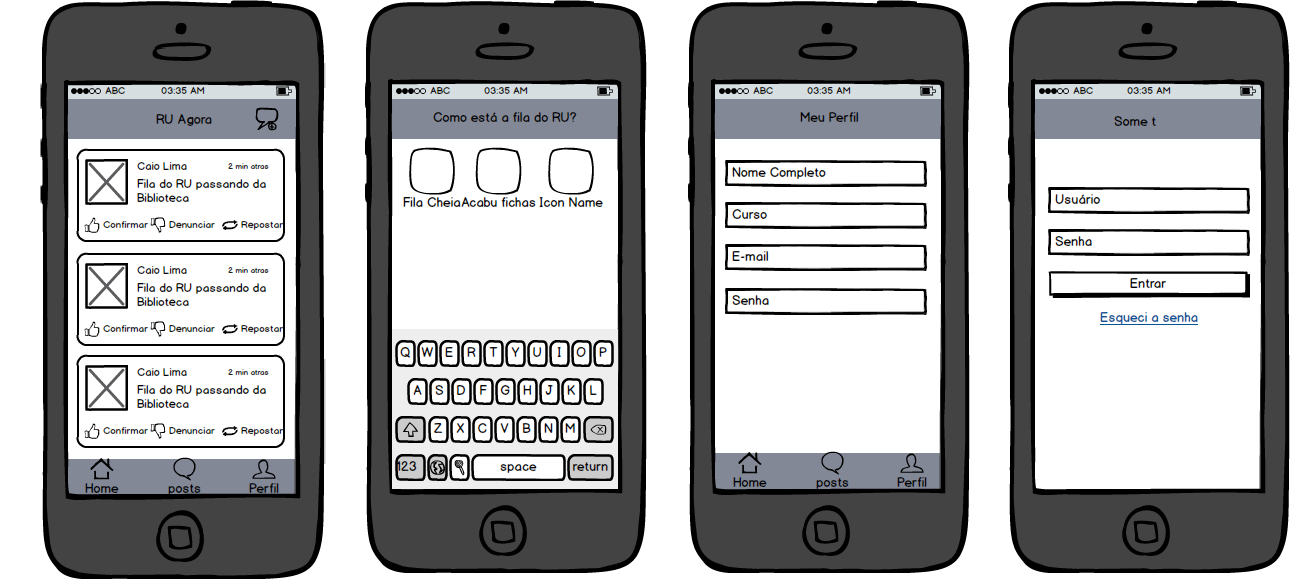
\includegraphics[width=.7\textwidth]{assets/img/home.png}
\caption{Esboço da interface do sistema voltado para smarthphones.}
\label{fig:mobilefig}
\end{figure}

\begin{figure}[ht]
\centering
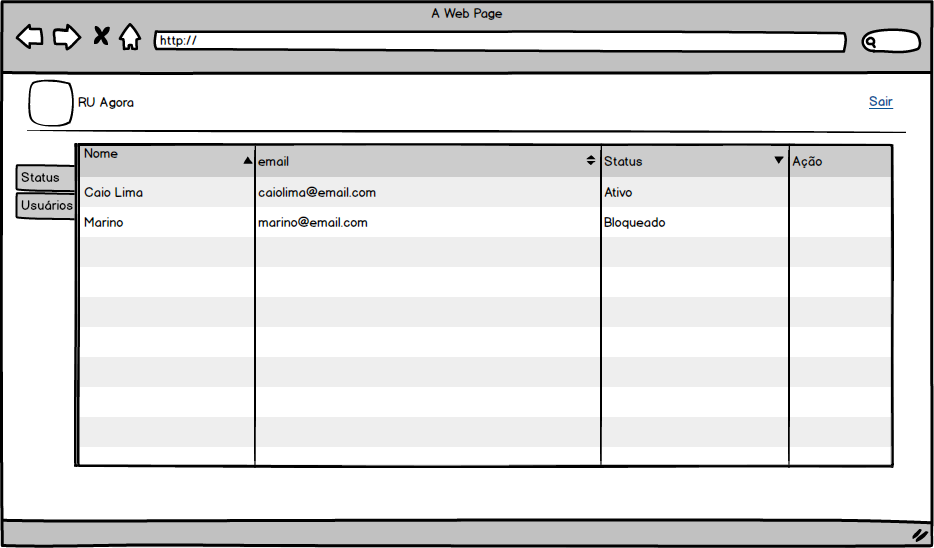
\includegraphics[width=.7\textwidth]{assets/img/mockup.png}
\caption{Esboço da interface do sistema web.}
\label{fig:webfig}
\end{figure}

\newpage
\section{Requisitos}

Requisitos funcionais

\subsection{Cadastrar nova conta}
Deve ser disponibilizado para novos usuários não autenticados, a possibilidade criação de uma nova conta.

\subsection{Logar no sistema}
Deve ser disponibilizado uma tela de login, onde o usuário possa se autenticar no sistema.

\subsection{Editar perfil}
Deve ser possível a um usuário logado no sistema, a possibilidade de editar seu próprio perfil.

\subsection{Informar status do RU}
Deve estar disponível para um usuário logado a possibilidade de informar um novo status do RU, dentre os listados na lista abaixo.

\begin{enumerate}

  \item Fila
  \begin{enumerate}
    \item Fila grande
    \item Fila pequena
  \end{enumerate}
  \item Fichas
  \begin{enumerate}
    \item Fichas acabaram
  \end{enumerate}
  \item Cardápio
  \begin{enumerate}
    \item Comida Muito Boa
    \item Comida razoável
    \item ``Só tem Soja viu bem?"
    \item ``Peixe"
    \item ``Fígado"
    \item ``Charutinho de soja"
    \item Contém anomalias.
  \end{enumerate}

\end{enumerate}

\subsection{Visualizar status do RU}
Deve estar disponível para um usuário logado a possibilidade de visualizar os status informados pelos demais usuários do sistema.

\subsection{Replicar status de outro usuário}
O usuário deve ser capaz de replicar o status informado por outro usuário, reforçando assim a relevância daquele status no sistema.

\newpage
\section{Arquitetura}

A arquitetura do sistema é divida em três camadas (fig.\ref{fig:arqfig}). Sendo a responsabilidade da primeira camada, a gerência da lógica da interface. A segunda é a camada de business, que
contém as regras de negócio das funcionalidades do sistema. E por fim, temos a camada persitance, que atua como intermediário entre a aplicação e a base de dados.

\begin{figure}[ht]
\centering
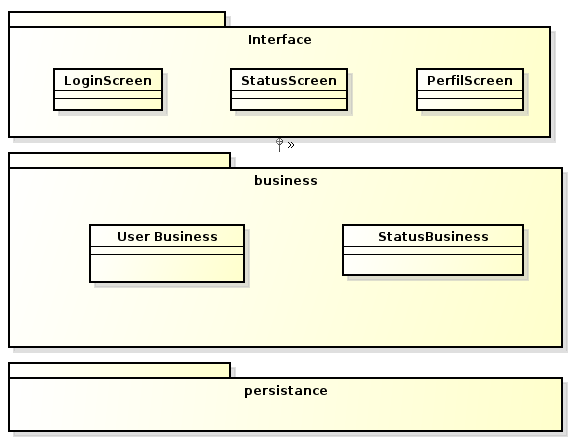
\includegraphics[width=.7\textwidth]{assets/img/arquitetura.png}
\caption{Arquitetura em três camadas do sistema.}
\label{fig:arqfig}
\end{figure}

\section{Casos de uso}

\begin{figure}[ht]
  \centering
  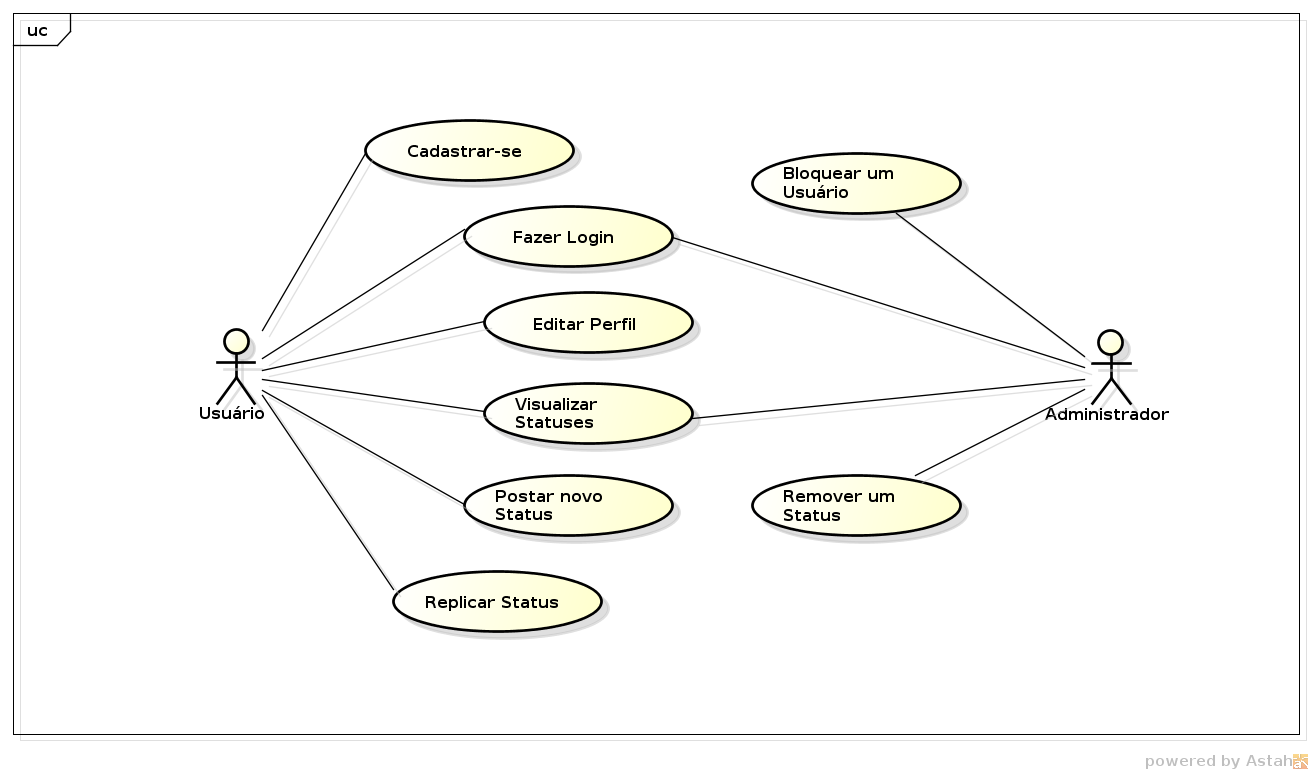
\includegraphics[width=.7\textwidth]{assets/img/useCases.png}
  \caption{Diagrama dos casos de uso.}
  \label{fig:usecasesfig}
\end{figure}

\subsection{UC01 -- Cadastrar-se}
\textbf{Atores:} Usuário \\
\textbf{Precondições:} O usuário deve possuir um e-mail \\
\textbf{Descrição:} O usuário se cadastra no sistema para poder utilizá-lo plenamente.

\textbf{Fluxo Normal}
\begin{enumerate}
  \item O usuário acessa o sistema
  \item O usuário clica em cadastrar-se
  \item O usuário preenche os campos solicitados pelo sistema
  \item O usuário aperta em ok
\end{enumerate}

\subsection{UC02 -- Fazer Login}
\textbf{Atores:} Usuário, Administrador \\
\textbf{Precondições:} O usuário deve possuir cadastro no sistema \\
\textbf{Descrição:} O usuário faz login com o seu cadastro no sistema, para poder utilizá-lo plenamente.

\textbf{Fluxo Normal}
\begin{enumerate}
  \item O usuário acessa o sistema
  \item O usuário aperta em Entrar
  \item O usuário preenche os campos de e-mail e senha
  \item O usuário aperta em Login

\end{enumerate}


\textbf{Fluxo de Excessão E1.}
\begin{enumerate}
  \item [4.1] Sistema reconhece as informações como inválidas e avisa ao usuário
    Retorna ao passo 2 do fluxo normal
\end{enumerate}

\subsection{UC03 -- Editar Perfil}
\textbf{Atores:} Usuário \\
\textbf{Precondições:} O usuário deve estar logado no sistema \\
\textbf{Descrição:} O usuário modifica informações do seu perfil (e-mail, senha, nome, foto, idade, sexo).

\textbf{Fluxo Normal}
\begin{enumerate}
  \item O usuário acessa o sistema
  \item O usuário aperta em Opções
  \item O usuário aperta em Editar Perfil
  \item O usuário preenche os campos com as novas informações
  \item O usuário aperta em Salvar
\end{enumerate}

\subsection{UC04 -- Visualizar Statuses}
\textbf{Atores:} Usuário, Administrador \\
\textbf{Precondições:} Nenhuma \\
\textbf{Descrição:} O usuário visualiza a lista de statuses postados por outros usuários. Não é necessário estar logado.

\textbf{Fluxo Normal}
\begin{enumerate}
  \item O usuário acessa o sistema
  \item O sistema mostra a lista de status ao usuário
\end{enumerate}

\subsection{UC05 -- Postar Novo Status}
\textbf{Atores:} Usuário \\
\textbf{Precondições:} O usuário deve estar logado no sistema \\
\textbf{Descrição:} O usuário envia um novo status ao sistema para que seja exibido na lista de status. Esse novo status será um dos modelos padrões disponibilizados pelo sistema.

\textbf{Fluxo Normal}
\begin{enumerate}
  \item O usuário acessa o sistema
  \item O usuário aperta em Novo Status
  \item O usuário seleciona um dos statuses padrões
  \item O usuário aperta em Enviar \\
\end{enumerate}

\subsection{UC06 -- Replicar Status}
\textbf{Atores:} Usuário \\
\textbf{Precondições:} O usuário deve estar logado no sistema \\
\textbf{Descrição:} O usuário envia uma réplica à um status postado por outro usuário.

\textbf{Fluxo Normal}
\begin{enumerate}
  \item O usuário acessa o sistema
  \item O usuário aperta no status a ser replicado
  \item O usuário aperta em Reply
  \item O usuário digita a sua réplica
  \item O usuário aperta em Enviar
\end{enumerate}

\subsection{UC07 -- Bloquear um Usuário}
\textbf{Atores:} Administrador \\
\textbf{Precondições:} O administrador deve estar logado no sistema \\
\textbf{Descrição:} O administrador bloqueia um usuário que infringiu as regras do sistema.

\textbf{Fluxo Normal}
\begin{enumerate} \item O administrador acessa o sistema
  \item O administrador acessa a lista de usuários
  \item O administrador seleciona o usuário a ser bloqueado
  \item O administrador aperta em Bloquear
\end{enumerate}

\subsection{UC08 -- Remover um Status}
\textbf{Atores:} Administrador \\
\textbf{Precondições:} O administrador deve estar logado no sistema \\
\textbf{Descrição:} O administrador remove um status que não segue as regras do sistema.

\textbf{Fluxo Normal}
\begin{enumerate}
  \item O administrador acessa o sistema
  \item O administrador seleciona o status a ser removido
  \item O administrador aperta em Apagar
\end{enumerate}


\section{Tecnologias utilizadas}


Para auxiliar no desenvolvimento do front-end da aplicação, utilizamos o framework Bootstrap. 
Decidimos usá-lo para a fim de acelerar o processo de criação de uma interface web responsiva aos
diferentes tamanhos de tela de dispositivos móveis. 

Para o back-end decidimos utilizar a linguagem de programação Ruby e seu framework para 
desenvolvimento de aplicações web, Rails. Essa escolha foi feita com base no conhecimento e interesse
dos integrantes do grupo, já que alguns possuem experiência desenvolvendo com essa linguagem e framework e os demais possuíam interesse em aprendé-la.


\section{Conclusão}

Portanto temos como finalidade, prover um sistema ágil capaz de disponibilizar
rápidos feedbacks para a comunidade, e pela comunidade. Com a informação à mão de forma mais veloz, 
a tomada de decisão dos frenquentadores em relação ao RU será potencializada, permitindo uma
economia de tempo, comodidade, além de possuir dados reais que espelhem a realidade vivenciada
pelos estudantes, para até mesmo cobrar, com um argumento mais forte, seus diretos aos responsáveis.
Portanto houve a necessidade de se construir uma aplicação responsiva que atendesse a necessidade 
desses usuários mobile.

%\section{References}
%
%Bibliographic references must be unambiguous and uniform.  We recommend giving
%the author names references in brackets, e.g. \cite{knuth:84},
%\cite{boulic:91}, and \cite{smith:99}.
%
%The references must be listed using 12 point font size, with 6 points of space
%before each reference. The first line of each reference should not be
%indented, while the subsequent should be indented by 0.5 cm.
%
%\bibliographystyle{sbc}
%\bibliography{sbc-template}

\end{document}
